\section{\orange{Discussion}}
In this section I will summarize key findings, and address the aims of the research.


what do we want from the model?
- it should not resample too often, about an eighth (this can be improved). of course we are counting the correct solutions too, over and over 
- it should be fast (when converged, it's immediate) (however everythong above depth 4 was critical)
- it should generalize OOD (it solves previously unseen tasks within and outside of task group)
- sleep is crucial

In the following section, I will compare FlowCoder to the concepts introduced in section [introduction or more specific 1.1, 1.2, etc.]

\subsection{\orange{Experimental Results}}

\begin{itemize}
    \item since the model solves most tasks within groups, it seeps to suggest that it learns relationships between groups (program space). 
\end{itemize}

The experiments of section \ref{sec:results} revealed that FlowCoder can be trained as an adequate program synthesizer. 
First, we found that the model solves more tasks in inference than in training, including tasks of groups which had previously been unseen, suggesting some out-of-distribution generalization capabilities.
Moreover, the model produces varied solutions, not only converging on a point estimate, the most likely program, but even in inference proposes multiple programs solving the tasks, suggesting that it has found a multi-modal distribution. 
In section [x] we have discussed why a multitude of representations are useful. In the context of program synthesis however, we must not conflate semantics with syntax [see discussion]. As shown in table \ref{tab:multiple_solutions}, many inefficient alternate solutions to a task were found. We would actually like to avoid programs that add 0, multiply by 1, etc. Breaking syntactic symmetries can be done by optimising for minimum description length and including an abstraction phase as is done in DreamCoder.
The model is able to sample varied correct solutions on the first step, suggesting that when we make the investment of training the model to convergence, we reap the benefits in the form of one-shot inference.
The model's performance steadily increases with alternating E-M steps, suggesting that it is beneficial to train the generative model separately from the forward policy and having the two models bootstrap each other. The generative model proposes better representations of the program space while the forward policy selects better actions, proportional to the posterior distribution, given the task at hand.


Many tasks have not been solved, but it looks like if the model had been kept training, it could converge on those too.
moreover, we need to adjust resampling since some tasks have not been solved but have been resampled many times.


- finding a balance between 
- exploration (beta, epsilon, fantasy) to find many modes, E-step
- exploitation (replay) converging on modes, not forgetting, M-step
and exploitation (exploration to find many modes) but also exploitation





Fijalkow et al. compare different search strategies and show that methods that do not use a machine-learned PCFG (e.g. depth-first search (DFS)) barely solve any tasks (max. 5) in over 1.5 hours \cite{fijalkow_scaling_2021}. [this should be in intro]


\begin{itemize}
    \item More tasks were solved in inference. since im going chronologically through the training set, the model doesn't see the first task ever again. this would be beneficial. minibatch sampling. 
    \item there are many other training strategies that could be employed.
    \item symmetry breaking. we want to avoid if True, or $+0$ or $*1$, etc.
\end{itemize}


\begin{itemize}
    \item benefit over dreamcoder etc. we can ask questions about partial programs. we are embedding programs as well as tasks, we can input a partial program into the model and ask what the next best step is. We can also train from partial tasks etc. making this method more dynamic. [to introduction?]
\end{itemize}



\begin{description}
    \item[Sampling strategy] ASTs can be constructed in various orders. Ideally, we could let the GFlowNet predict which node to expand. However, this would have meant creating an additional model as a node predictor, which increases FlowCoder's complexity. Moreover, since ASTs are inherently two dimensional and I am using a transformer to encode CFG rules as a representation of a program, ASTs have to be linearized. I decided to expand the tree in order of depth-first, both to eliminate the need for another model and also to give the transformer the input in consistent order, making learning easier. 
    \item[] - bottom-up construction could be beneficial as nodes can already be evaluated
    - construction order
    - include diagram
\end{description}










% Similar to both approaches, I am separating the generative model from the recognition model

DreamCoder enforces parsimonious programs during abstraction. Common patterns are refactored, shortening the programs. Deepsynth enforces programs of minimum description length by optimising for the expected number of programs before finding a correct solution. This works, if programs are considered in order of increasing length. Both of these methods however optimise for point estimates, i.e. the most likely program for a given task. Instead, I want to learn the posterior distribution, i.e. all solutions to a task, which of course is much harder.
I do this, first, because if we see that the model finds the posterior, it can always be simplified to MAP. Second, given the analogy of humans understanding the world via program-like concepts, we know that we can represent the world in various ways and we can find multiple solutions to a problem. Consider the following example: the task 
% [2,,6,8] -> 
% [1,2,3] -> [2,4,9]
% Surfaces and Essences analogy example abc:xyz :: abd: (wyz/ xya) 
% [123][987]
% abc xyz
% abd wyz/ xya


I constrain the program depth to 3, which is enough to solve most programs and is not too computationally heavy.
Since most tasks can be solved by short programs, 
Despite the minimum description length being a factor which may be necessary, I relax this condition






\subsection{\orange{Comparison to DreamCoder}}


\subsection{\orange{Speed}}
It is somewhat difficult to compare the time efficiency of my method with other approaches for various reasons. 
Both DeepSynth and DreamCoder predict weights for the PCFG and then parallelize search processes on multiple CPUs. DreamCoder train their model for about a day on 20-100 CPUs and it takes around 10 wake-sleep cycles to converge in the list domain. I instead am working on one GPU (with possible interruptions from other users on the cluster). DreamCoder shows that the refactoring algorithm used in abstraction is crucial in the list processing tasks, which I did not implement.
DeepSynth does not include model query time in their computations.
I am training my model on a filtered set of the original DreamCoder dataset, making it difficult to compare with DreamCoder and some of the DeepSynth experiments. 

[Moreover, I did not work too much on time optimizations and still it seems that it isnt too slow in a rough comparison with those other methods.]









\subsection{\green{Scaling the Model}}

\todo[inline]{check this, check what is necessary}

The time complexity for encoding an IO pair is \(\mathcal{O}(n)\), where \(n\) is the length of the IO pair. 

Similarly, the RuleEncoder's time complexity is \(\mathcal{O}(n)\) where \(n\) is the number of rules.

In each step of the trajectory, I embed the task and the current state, and use the transformer to construct the trajectory until completion. 

The transformer's complexity is \(O(num\_layers \times (d_{model}^2 \times n_{seq} + n_{seq}^2 \times d_{model}))\), where \(num\_layers\) is the number of layers, \(d_{model}\) is the model dimension, and \(n_{seq}\) is the sequence length.

The linear layers within the forward policy $\pi_\theta$ and partition function $Z_\theta$ have a complexity of \(O(d_{model}^2)\) due to the matrix multiplication involved.

The overall time complexity of a forward pass through FlowCoder is dominated by the transformer's complexity, which is \(O(num\_layers \times (d_{model}^2 \times n_{seq} + n_{seq}^2 \times d_{model}))\).

Since I have linearized the construction procedure, I reconstruct the list back to AST format and then evaluate the tree to get the program output.

The reconstruction and evaluation are both recursive processes that depend on the depth of the tree and number of arguments in each partial program. 
The worst-case complexity of program reconstruction, as well as the evaluation can be approximated as \(O(k^d)\), where \(d\) is the depth of the recursion, which corresponds to the length of the program list, and \(k\) is the average number of arguments for each function in the program. In my experiments only one argument per function is allowed.

[sec x to see how we can mitigate this (better program representation, construction, evaluation (instead of reconstruction, reformating etc. ))]
In general i want to show that the model scales. 

Subsequently, I compute the reward.

The Levenshtein edit distance algorithm, when implemented using dynamic programming, has a time complexity of 
$\mathcal{O}(m \times n)$, where $m$ and  $n$ are the lengths of the two input strings.
\subsubsection{Scaling}
\begin{itemize}
    \item Scaling the model (How does the model scale with larger CFGs?)
    \item We need to show that with abstraction, we could theoretically scale
    \item Scaling neural search paper
    \item how would it work using GFNs
    \item how would it work if we use abstraction like in DC? DC shows it is scalable.
    \item this needs to be related to increasing number of primitives, maybe look at dreamcoders complexity. we save complexity by not having to search, and also space, since we dont have to save anything, we just need to train a phat model
\end{itemize}
    


The scalability of the model depends on various factors. First, we have seen that GFN can deal with the marginalization term and is an instance of amortized bayesian inference. This means that we can capitalise on seen data to generalise to many modes even in high-dimensional spaces. [show that amortized inference scales]
The intention of this study is to show that the general method of using GFNs for program synthesis is useful and not to optimise it for efficiency and scalability. Many adjustments can be made to accommodate for scaling. 
program representation, 
choosing the generative and forward (and possibly backward) policy models, 
parallelizing tasks,
different training strategies
most importantly, as discussed in [sec DreamCoder], the abstraction phase is crucial to narrow the depth of the search tree. (and MDL). 
The end-goal is to have an increasing DSL as well. 
Scaling neural search paper
all of the program construction/ reconstruction/ evaluation can be reduced. 


the problem with scaling is marginalization. DC deals with this by marginalising over a beam of programs for each task. GFN deals with it by adhering to the flow objective. 
other amortized variational inference methods, \dots






















\subsection{\orange{program representation}}
Other ideas to represent ASTs are GNNs, or Tree-Transformers [which were explored, but the computational complexity gets higher [source]. also distributed representations of aggregations are an option like in GFN-EM.], however, I settled on using a regular transformer, since it has been shown that it can learn tree structures implicitly, through positional encoding and also [source] show that the performance is similar.
since we are representing trees, it might be beneficial to embed programs in hyperbolic space [see conceptual spaces]. 
There are other ways to embed the cfg, [e.g. see kim].
- 3-index bigram, .. compound PCFG including information of neighboring states, parents, childrewn, etc. 



since we are representing the tree as an array of rules, so that we can use them with transformer, we need to reformat it back into a tree to evaluate it. i.e. we need to fisrt construct it and then go through it again for evaluation. this slows down the computation. 


- heapsearch, evaluation, using sub-trees, etc. 
Another expansion is using a depth first search (DFS) [source] approach (note that this is not about searching through the CFG, but constructing the AST). Since we are essentially linearising a tree when giving it as input to the transformer, the transformer has additional order information, which in combination with positional encoding lets it learn better. 

hyperbolic space



We could embed parent, child, etc. to make ean embedding of a rule more informed. i chose not to do it to see whether its enough (discuss in limitations,e tc. )

Syntax vs Semantics 
Semantics can be understood as data flow, e.g. partial evaluations could be used as part of the representation of the program. 
type information 
For a discussion on semantics and meaning see sec [meaning]
In LLMs, we see that they l









\subsection{\red{Program Embeddings}}
programs are commonly represented as AST. 
% Although these models are great, their method reveals a foundational limitation: their heavy reliance on syntactical constraints. While these constraints are undoubtedly vital for ensuring the correctness of generated programs, they do not necessarily guarantee a deep understanding or utilization of semantic relationships within the code. 
% A lot of information may be lost, by disregarding the semantic relationships. As we have seen in [reference LLMs], there seems to be a semantic grammar on top of the syntactical structure of the language which we may be able to leverage.
% This has been criticized in [cite all the relevant papers (using GNNs, etc. ) also Kim's neural PCFG].
% Perhaps we can utilise transformers to learn a "program space", a kind of neural probabiilistic context-free grammar

% - we could imagine a program space in which symmetries [reference] and so on could be leveraged. For example, one could argue that "\(+\)" is to "\(-\)" as "\(\div\)" is to "\(\times\)", and anyways once we create programs which really represent actual concepts, the same regularities should be systematically compressed.

Does DC learn a program space (discuss their tsne)
- hyperbolic

Graph Neural Networks seem like an interesting option to represent ASTs
Allamanis et al. use Gated Graph Neural Networks to include local semantics in their program representations 

Allamanis et al. use Gated Graph Neural Networks to represent both syntactic and semantic information by including data flow and type hierarchy signals \cite{allamanis2017learning}. The authors formalize how to turn ASTs to graphs.

Wang et al. propose a semantic program embedding, learnt from program execution traces \cite{wang2017dynamic}.

Ibarz et al. present a generalist neural algorithmic learner by leveraging GNNs \cite{ibarz2022generalist}.
Zhang et al. propose a novel neural AST representation of source code \cite{zhang_novel_2019}.

Oliviera and Löh develop abstract syntax graphs (rather than trees) to preserve sharing and recursion within a DSL \cite{oliveira_abstract_2013}.









\subsection{\red{reward}}

\begin{itemize}
    \item Reward should be learnt (Energy based model). Where does the brain get it from?
    \item Is Levenshtein a reasonable reward? think about computational complexity (Kolmogorov complexity)
    \item Reward depends on tasks
    \item Rewards can be based on utility or efficiency rather than accuracy, or on aesthetics or other determinants. This is a complex topic which should be investigated in the future. 
\end{itemize}






\subsection{\red{Limitations}}
\begin{itemize}
    \item Make the network choose where to expand (not DFS). Note that we are not going through the CFG DFS, but creating the AST with DFS (GNN, evaluation etc. )
    \item What should be the best order of solving tasks? should we try to solve a certain task for x amount of time and then move on to the next? curriculum learning? 
    \item Better reward
\end{itemize}









\subsection{\red{Related Work}}
\begin{itemize}
    \item apperception engine
    \item one language to rule them all
    \item 
\end{itemize}

\subsection{\red{Future Work}}
\begin{itemize}
    \item testing sleep, exploration, etc. 
    \item Sub-trajectory balance
    \item Learning from dataset of good programs (akin to someone telling you a solution)? 
    \item Train from middle of states
    \item Train backward policy, then we can also see finished states and predict trajectories that led to them
    \item caching evaluations, bottom-up
    \item we could let automate how long to train. if it is solving the task in 100 consecutive e steps and also in m stepts, it could also just move on. 
    \item Hyberbolic space (relate to holarchies)
\end{itemize}
































\subsubsection{\orange{Comparison to other approaches}}

Previously, techniques in approximate Bayesian inference, have been applied to deal with the difficult marginalization term.

Variational Inference (VI) is a strategy that leverages a simpler distribution \( q(z | x) \)  to approximate a more complex target distribution. This is achieved by minimizing the Kullback-Leibler (KL) divergence, a similarity measure of probability distributions, between the true distribution and its approximation.

\[
    D_{KL}[q(z|x) || p(z|x)]
\]

The approximation can be optimized by increasing the Evidence Lower Bound (ELBO) by:

\begin{equation}
\text{ELBO} = E_{q(z|x)}[\log p(x|z)] - D_{KL}(q(z|x) || p(z|x))
\end{equation}
Where \( E_{q(z|x)} \) denotes the expectation under the recognition density \( q \).

In the context of \emph{amortized} VI, computation of the variational parameters \( \phi \) is shared across multiple data points. Traditional VI might determine a unique set of variational parameters \( \phi_i \) for each data point \( x_i \), which is computationally intensive. Amortized VI, however, leverages a function (commonly a neural network) to compute the variational parameters \( \phi \) for any data point \( x \) in a single pass, enhancing efficiency. In other words, we parameterize the recognition density. 

this aligns with the free energy principle formulation [show that.]
maximizing the evidence lower bound (ELBO), is equivalent to the negative free energy. 

Amortized variational inference refers to the use of a parameterized function (e.g., a neural network) to approximate the posterior distribution in a variational Bayesian setting, where the parameters are learned once and can be used to infer the posterior for any given data point without retraining. It is "amortized" because the cost of learning the inference model is spread over all the data points it is used on.

GFlowNets relate to amortized variational inference in the sense that they learn a policy network that can generate samples for any given reward function without having to solve a new optimization problem for each sample. This is similar to how an amortized inference model can be applied to new data without additional optimization.

In both cases, the "amortization" allows for efficient inference or generation after the initial cost of learning the model. However, GFlowNets focus on learning to sample in proportion to a reward function, whereas amortized variational inference is concerned with approximating the posterior distribution of latent variables given observed data.

\begin{itemize}
    \item Relation to MDPs, POMDPs
    \item Relation to Reinforcement learning
    \item Relation to MCMC sampling
    \item Relation to Variational inference. 
\end{itemize}


variational approximation we need an ELBO but with GFNs we don't 

A variety of techniques have emerged in the domain of program synthesis, [each with pros and cons].

Ullman et al. MCMC[source, definition] and Metropolis-Hastings[source, definition] \cite{ullman_theory_2012}. [include pros and cons]

% Example-based synthesis draws inspiration from how humans often learn—from examples. These methods generate programs by generalizing from provided instances, which mirrors pedagogical processes and experiential learning [source].

% Stochastic Search: By randomly exploring the space of possible programs, these methods mirror heuristic-based cognitive processes. Genetic algorithms, for instance, mimic evolutionary processes to evolve optimal or near-optimal solutions.

% Neural Program Synthesis: Neural networks, especially recurrent ones, have shown promise in generating programmatic structures. The parallels between neural networks and neural structures in the brain offer tantalizing possibilities for cognitive science.


% A variety of statistical techniques have been proposed, ranging from evolutionary algorithms, 
% machine learning and genetic programming to MCMC sampling and probabilistic inference [source].  

% Machine learning techniques can be used to augment other search methodologies based on enumerative search or deduction by providing likelihood of various choices at any choice point. One such choice point is selection of a production for a non-terminal in a grammar that specifies the underlying program space. The likelihood probabilities can be function of certain cues found in the input-ouput examples provided by the user or the additionally available inputs [89]. These functions are learned in an offline phase from training data. 

% Genetic programming is a program synthesis method inspired by biological evolution [72]. It involves maintaining a population of individual programs, and using that to produce program variants by leveraging computational analogs of biological mutation and crossover. Mutation introduces random changes, while crossover facilitates sharing of useful pieces of code between programs being evolved. Each variant's suitability is evaluated using a user-defined fitness function, and successful variants are selected for continued evolution. The success of a genetic programming based system crucially depends on the fitness function. Genetic programming has been used to discover mutual exclusion algorithms [68] and to fix bugs in imperative programs [146] 

% MCMC sampling has been used to search for a desired program starting from a given candidate. The success crucially depends on defining a smooth cost metric for Boolean constraints. STOKE [124], a superoptimization tool, uses Hamming distance to measure closeness of generated bit-values to the target on a representative test input set, and rewards generation of (almost) correct values in incorrect locations. 

% Probabilistic inference has been used to evolve a given program by making local changes, one at a time. This relies on modeling a program as a graph of instructions and states, connected by constraint nodes. Each constraint node establishes the semantics of some instruction by relating the instruction with the state immediately before the instruction and the state immediately after the instruction [45]. 

% Belief propagation has been used to synthesize imperative program fragments that execute polynomial computations and list manipulations [62].

\todo[inline]{should the above be in the intro??}







\subsubsection{\red{Biological Plausibility}}
\begin{itemize}
    \item Why are/ aren't types plausible? Related to categories?
    \item CFG? where does it come from?
    \item primitives?
    \item Discuss Abduction, etc. 
    \item of course a model that can create programs of depth 3 is somewhat underwhelming when compared to human cognition. 
\end{itemize}









































\subsection{\red{Conclusion}}
\begin{itemize}
    \item The conclusion here is that GFN is a viable method for program synthesis which could replace models such as DC. 
    \item 
\end{itemize}






























% GFlowNets can be seen as extending the already rich family of **amortized variational inference** methods, more specifically amortized hierarchical variational inference, where there are several latent variables $s_1, s_2, \ldots$ and they are hierarchically organized so that when we generate an object $x$ we start by sampling $s_1$, then $s_2|s_1$, then $s_3|s_2$, etc and then convert the last $s_{n-1}$ into $x=s_n$ with a model $P(s_1,s_2,\ldots,s_{n-1},x)=P(x|s_{n-1})P(s_{n-1}|s_{n-2})\ldots P(s_2|s_1)$. As discussed in [[7]](https://www.notion.so/The-GFlowNet-Tutorial-95434ef0e2d94c24aab90e69b30be9b3?pvs=21) and [[9]](https://www.notion.so/The-GFlowNet-Tutorial-95434ef0e2d94c24aab90e69b30be9b3?pvs=21), the sequence $\tau=s_1,\ldots,s_{n-1},x$ corresponds to the GFlowNet trajectory $\tau$, with $P_F(\tau)=P(x|s_{n-1})\ldots P(s_2|s_1)$. As with other variational inference approaches one also learns an inference machine $Q(\tau|x)$ which corresponds to $P_B(\tau|x)$ in GFlowNets. With variational method we also have a marginal data distribution (which we could denote $Q(x)$) that with GFlowNets corresponds to the normalized reward function $R(x)/Z$ that can be queried as needed by the training procedure (unlike a fixed dataset). Another difference is that variational methods are trying minimize the reverse KL divergence between $Q$ and $P$ (or using importance sampling, the forward KL) whereas GFlowNets are trained with a diversity of losses, e.g. corresponding to something like $(\log Q(\tau) - \log P(\tau))^2$ with Trajectory Balance, that open the possibility of offline training (with trajectories $\tau$ sampled from a distribution different from the online samples from $Q$). In [[9]](https://www.notion.so/The-GFlowNet-Tutorial-95434ef0e2d94c24aab90e69b30be9b3?pvs=21), we show that when a GFlowNet is trained with trajectory balance on-policy, the expected gradient is the same as with variational inference and the reverse KL, but the variance is different (and the trajectory balance gradient is equivalent to using a variance reduction trick, compared with regular variational inference). The typical variational inference objective (the ELBO or reverse-KL) leads to mode-following (focussing on one mode) and the forward KL leads to mean-following (overly conservative, sampling too broadly) and annoying variance when implemented with importance sampling. Instead the off-policy GFlowNet objectives (e.g., with a tempered version of $P_F$ as training policy) seem to strike a different balance and tend to recover more of the modes without the down-side of the forward-KL variational inference variants (mean-following and high variance gradients). Another difference is that GFlowNets can learn flows and conditional flows, which correspond to marginalized quantities, as discussed [above](https://www.notion.so/The-GFlowNet-Tutorial-95434ef0e2d94c24aab90e69b30be9b3?pvs=21).




\begin{itemize}
    \item Robustfill
    \item DeepCoder
    \item Etc.
    \item Paved the way in a coubple of different ways, etc.
\end{itemize}















\begin{figure}
    \centering
    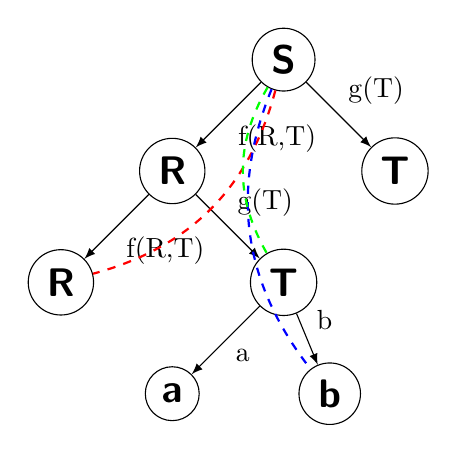
\begin{tikzpicture}[
      node distance = 2cm,
      auto,
      block/.style = {circle, draw, font=\sffamily\Large\bfseries},
      line/.style = {draw, -latex}
    ]
    
    % Nodes
    \node [block] (S) {S};
    \node [block, below left of=S] (R1) {R};
    \node [block, below right of=S] (T1) {T};
    \node [block, below left of=R1] (R2) {R};
    \node [block, below right of=R1] (T2) {T};
    \node [block, below right of=R2] (a) {a};
    \node [block, right of=a] (b) {b};
    
    % Paths
    \path [line] (S) -- node {f(R,T)} (R1);
    \path [line] (S) -- node {g(T)} (T1);
    \path [line] (R1) -- node {f(R,T)} (R2);
    \path [line] (R1) -- node {g(T)} (T2);
    \path [line] (T2) -- node {a} (a);
    \path [line] (T2) -- node {b} (b);
    
    % DFS, BFS, A* paths (without specific details)
    \draw [red, thick, dashed] (S) to [bend left] (R2);
    \draw [blue, thick, dashed] (S) to [bend right] (b);
    \draw [green, thick, dashed] (S) to [bend right] (T2);
    
    \end{tikzpicture}
    \caption{Illustration of the tree of leftmost derivations.}
    \end{figure}


    % \begin{figure}
    %     \centering
    %     \begin{tikzpicture}[
    %       node distance = 1.5cm,
    %       auto,
    %       block/.style = {circle, draw, fill=orange, font=\sffamily\Large},
    %       line/.style = {draw, -latex},
    %       dashedline/.style = {dashed, -latex}
    %     ]
        
    %     % Legend
    %     \node [draw, rectangle, minimum width=3cm, minimum height=2cm, font=\small] at (0,5) {legend};
    %     \node [font=\small] at (0,4.5) {--- semantic equivalence};
    %     \node [font=\small] at (0,4) {⊔ nondeterministic choice};
        
    %     % Nodes for (A)
    %     \node [block] at (0,2) (A1) {+};
    %     \node [block, below left of=A1] (A1L) {5};
    %     \node [block, below right of=A1] (A1R) {x};
        
    %     % Nodes for (B)
    %     \node [block] at (4,2) (B1) {+};
    %     \node [block, below left of=B1] (B1L) {5};
    %     \node [block, below right of=B1] (B1R) {x};
        
    %     % Paths for (A)
    %     \draw [line] (A1) -- (A1L);
    %     \draw [line] (A1) -- (A1R);
        
    %     % Paths for (B)
    %     \draw [dashedline] (B1) -- (B1L);
    %     \draw [dashedline] (B1) -- (B1R);
        
    %     % ... continue for other nodes and paths ...
        
    %     \end{tikzpicture}
    %     \caption{Refactorings and data structure.}
    %     \end{figure}



    \begin{figure*}[htbp]
        \centering
        \begin{adjustbox}{width=\textwidth}
            \begin{tikzpicture}[level distance=1.5cm,
                level 1/.style={sibling distance=6cm},
                level 2/.style={sibling distance=3cm},
                every node/.style={circle, draw}]
            
            \node at (-9,0) {$\lambda$};

            \node at (-6,0) {$\lambda$}
                child {node {+}};
            \node at (-3,0) {$\lambda$}
                child {node {+}
                    child {node {x}}
                };
            \node at (0,0) {$\lambda$}
                child {node {+}
                    child {node {x}}
                    child {node {x}}
                };
            \node at (3,0) {$\lambda$}
                child {node {+}
                    child {node {x}}
                    child {node {max}
                        child {node {x}}
                        child {node {x}}
                    }
                };
            \node at (6,0) {$\lambda$}
                child {node {+}
                    child {node {x}}
                    child {node {max}
                        child {node {x}}
                        child {node {y}}
                    }
                };
            \node at (9,0) {$\lambda$}
                child {node {+}
                    child {node {x}}
                    child {node {max}
                        child {node {y}}
                        child {node {x}}
                    }
                };
            
            % Second tree sequence (Figure 6)
            \node at (-3,-5) {+};
            \node at (0,-5) {+}
                child {node {pow}};
            \node at (3,-5) {+}
                child {node {pow}
                    child {node {y}}
                };
            \node at (6,-5) {+}
                child {node {pow}
                    child {node {y}}
                    child {node {x}}
                };
            \node at (9,-5) {+}
                child {node {pow}
                    child {node {y}}
                    child {node {x}}
                }
                child {node {3}};
            
            \end{tikzpicture}
        \end{adjustbox}
        \caption{Creation of trees showing the construction process.}
    \end{figure*}
    
    













